%=========================================================================
% (c) Michal Bidlo, Bohuslav Křena, 2008

\chapter{Úvod}
Tvorbou počítačových her se zabývá celé odvětví průmyslu. Pracují na nich mnohačlenné vývojářské týmy, i přes to se vyvíjí měsíce a roky. Ale co vše je vlastně  potřeba vytvořit, abychom se mohli projít ve virtuální 3D scéně? Právě na tuto otázku by měla tato bakalářská práce reagovat. Tato bakalářská práce by měla popsat implementaci jednoduché hry, dema, ovšem veškerá implementace bude směřována k případnému pozdějšímu rozšíření do~plné hry. Vše bude řešeno buď vlastní implementací nebo \emph{freeware/open-source} knihovnami.
Práce se bude zabývat realizací základního osvětlení, načtení a vykreslení modelů, interakcí s uživatelem, dále vyřešením kolizí pomocí externí knihovny. K těmto cílům budou použity knihovny založené na \emph{OpenGL}, jmenovitě \emph{Assimp}\cite{assimp} pro načítání, \emph{Bullet physic engine}\cite{bullet} pro zachytávání kolizí a fyzikální model a \emph{irrKlang}\cite{irrKlang} pro ozvučení a knihovny \emph{glew\cite{glew}, glfw\cite{glfw}, glm\cite{glm}} pro základní práci s grafikou. Inspirací mi byly knihy Moderní počítačová grafika\cite{MPGBook}, 3D Game Engine Desight od David H. Eberly\cite{gengine} a OpenGl Průvodce programátor\cite{OpenGLBookcz}.          

\chapter{Teorie}
V této kapitole bude popsána netriviální teorie, která bude později použita ve výsledné aplikaci. Primárně se zaměří na teorii implementovanou mnou, nikoliv na teorii obsaženou v~knihovnách třetích stran. Hlavním zdrojem pro tuto kapitolu bude sloužit kniha Moderní počítačová grafika\cite{MPGBook}. 
\section{Phongův osvětlovací model}
Phongův osvětlovací model předpokládá, že většina světla nedopadá do kamery přímo, ale odrazem od objektů.
Toto odražené světlo se dělí na tři složky \emph{ambientní}, \emph{difuzní} a \emph{spekulární}. Kde \emph{ambietní} složka představuje světlo rovnoměrně rozptýlené v prostoru, tedy osvětluje všechny fragmenty stejně. \emph{Difuzní} složka, pak představuje světlo od zdroje  přímo dopadající na fragment. Intenzita osvětlení \emph{difuzní} složkou se odvíjí od úhlu dopadu. Čím blíže k normále, tím více je fragment osvětlen. Poslední složka, \emph{spekulární} neboli zrcadlová, představuje světlo odrážející se od fragmentu do kamery. Tedy její intenzita se mění na základě polohy kamery vůči úhlu dopadu světla tzn. jak moc se světlo odráží směrem ke~kameře. Phongův model v tomto případě předpokládá ideální odraz, tedy úhel dopadu se rovná  úhlu odrazu. Intezitu celkového ovětlení fragmentu lze obecně spočítat vzorcem:
\begin{equation}\label{phong}
I_V = I_A \vec{r_a} + \sum_{k=1}^{N}I_{L_k}[r_s(\vec{v}\cdot\vec{r_k})^h + r_d(\vec{l_k}\cdot\vec{n})]\cite{MPGBook}
\end{equation}
Vzorec \ref{phong} je obecný pro \emph{N} zdrojů světla. V aplikaci bude využíváno jako zdroje světla pouze slunce, pak tedy lze vzorec zjednodušit na:
\begin{equation}\label{MyPhong}
I_V = I_A r_a + r_s(\vec{v}\cdot\vec{r_k})^h + r_d(\vec{l_k}\cdot\vec{n})
\end{equation}
 V obou vzorcích přestavuje $ I_A $ intenzitu \emph{ambientní} složky a $r_a$ její barvu. V prvním vzorci se pak sčítají všechny \emph{difuzní} a \emph{spekulární} složky všech zdrojů světla. V případě této bakalářské práce se tím pádem suma redukuje pouze na jeden vzorek.

\section{Shadow depth map}\label{shadowMap}
\emph{Shadow depth map}, českým ekvivalentem stínová paměť hloubky\cite{MPGBook}, je algoritmus na výpočet vlastních i vržených stínů hmotných těles. Vyznačuje se vysokou rychlostí výpočtu a nízkou kvalitou stínů, vyšší paměťovou náročností pro více zdrojů světla. Algoritmus spočívá ve vytvoření hloubkové mapy, podobně jako při řešení viditelnosti pomocí \emph{z-buffer} algoritmu, kdy je v mapě uložená vzdálenost nejbližšího bodu ke zdroji světla. Při vykreslování se porovná hloubka daného bodu s hodnotou v mapě. Pokud je daná hodnota vyšší, pak je fragment ve stínu, jestliže je ale nižší, tak ve stínu není. V důsledku použití rastrové mapy se u tohoto algoritmu projevují všechny problémy spojené s mapováním textur, jako například \emph{aliasing}, problémy s rozlišením mapy. Dále může v důsledku nepřesnosti rasterizace vzniknout jemná odchylka. Následkem toho hloubka bodu vyjde o něco větší, než při zápisu do hloubkové mapy a začne vrhat stín sám na sebe. Algoritmus této metody se dá zapsat jako: 
\\
\\ 

\lstset{frame = single, language=C++, framexleftmargin=15pt,label="Algoritmus"}

\begin{lstlisting}[caption=Algoritmus Shadow depth map]
for(int i=0;i<countOfLight;i++){
	drawToShadowMap(&shadowBuffer[i]);
}
draw()
//in fragment shader -- for each fragment
in vec3 coord // coordinate of fragment

// matrix for transform from model space to lightspace
uniform mat4[] LightMVP;	
// array of shadow depth map
uniform sampler2DShadow ShadowSampler[];

// array of structur for light, function getLight
// return sum of ambient, diffuse and specular part
uniform lightSource light;

vec3 sum(0,0,0);
for(int i=0;i<countOfShadowMaps;i++){
	L-coord = LightMVP[i] * coord;
	float depth =texture2D(ShadowSampler[i], L-Coord.xy);
	if(depth<L-Coord.z+0.0001){
		sum += 0.5 * getLight(light[i]);
	}else{
		sum += getLight(light[i]);	
}
	
\end{lstlisting}\label{SDM-alg}
Algoritmus \ref{SDM-alg} je psán v podstatě v \emph{glsl}, ale tento jazyk poskytuje i funkci přímo pro provední porovnání s hodnotou v \emph{shadow map} \emph{texturProj(shadowMap,lightCoord)}. Ovšem to by nebylo moc názorné.
\section{Skeleton animation}\label{SA}
\emph{Skeleton animation }je metoda inspirovaná stavbou lidského těla. To znamená, že společně s~kostí se vždy pohybuje i od ní celá pokračující část těla. Příkladem může být pohyb stehenní kosti, který způsobí následný pohyb i kosti holení, lýtkové, kostmi kotníku a celého chodidla. Základní \emph{Skeleton animation} využívá dvě vrstvy, síť bodů jako kůži a stromovou strukturu kostí viz. obrázek \ref{skeletalAnimation}.
Pokud je potřeba realističtějšího chování, používají se komplikovanější verze, kdy mezi vrstvou vrcholů a kostí je ještě jedna nebo dokonce několik vrstev simulující svalstvo. Toto vylepšení zabraňuje vzniku zlomů v kůži, či prolnutí vrcholů z jedné strany na druhou.

Ovšem pro potřeby implementace této práce dostačuje základní varianta, neboť výše zmíněné vady se projevují primárně u modelů s rotacemi o velký úhel. Pro jednoznačný popis a vykreslení jednoduché varianty \emph{Skeleton animation} je potřeba znát:
\begin{itemize}
	\begin{item}
		pro vrchol:
			\begin{itemize}			
			\item pozici, uv souřadnice, normálu
			\item seznam kostí, kterými je ovlivněn
			\item seznam vah, poměr ovlivnění, pro tyto kosti
		\end{itemize}
	\end{item}
	\begin{item}
	pro kost:
	\begin{itemize}
		\item transformační matici pro přechod ze souřadní soustavy kosti do soustavy bodů, dále nazývána offsetová matice nebo matice odsazení 
	\end{itemize}

\end{item}
	\begin{item}
	pro uzel:
	\begin{itemize}
		\item transformační matici pro přechod ze soustavy tohoto uzlu do soustavy rodičovského uzlu pro každý klíčový snímek animace
	\end{itemize}
	
\end{item}
	
\end{itemize}  
\begin{figure}
\begin{center}

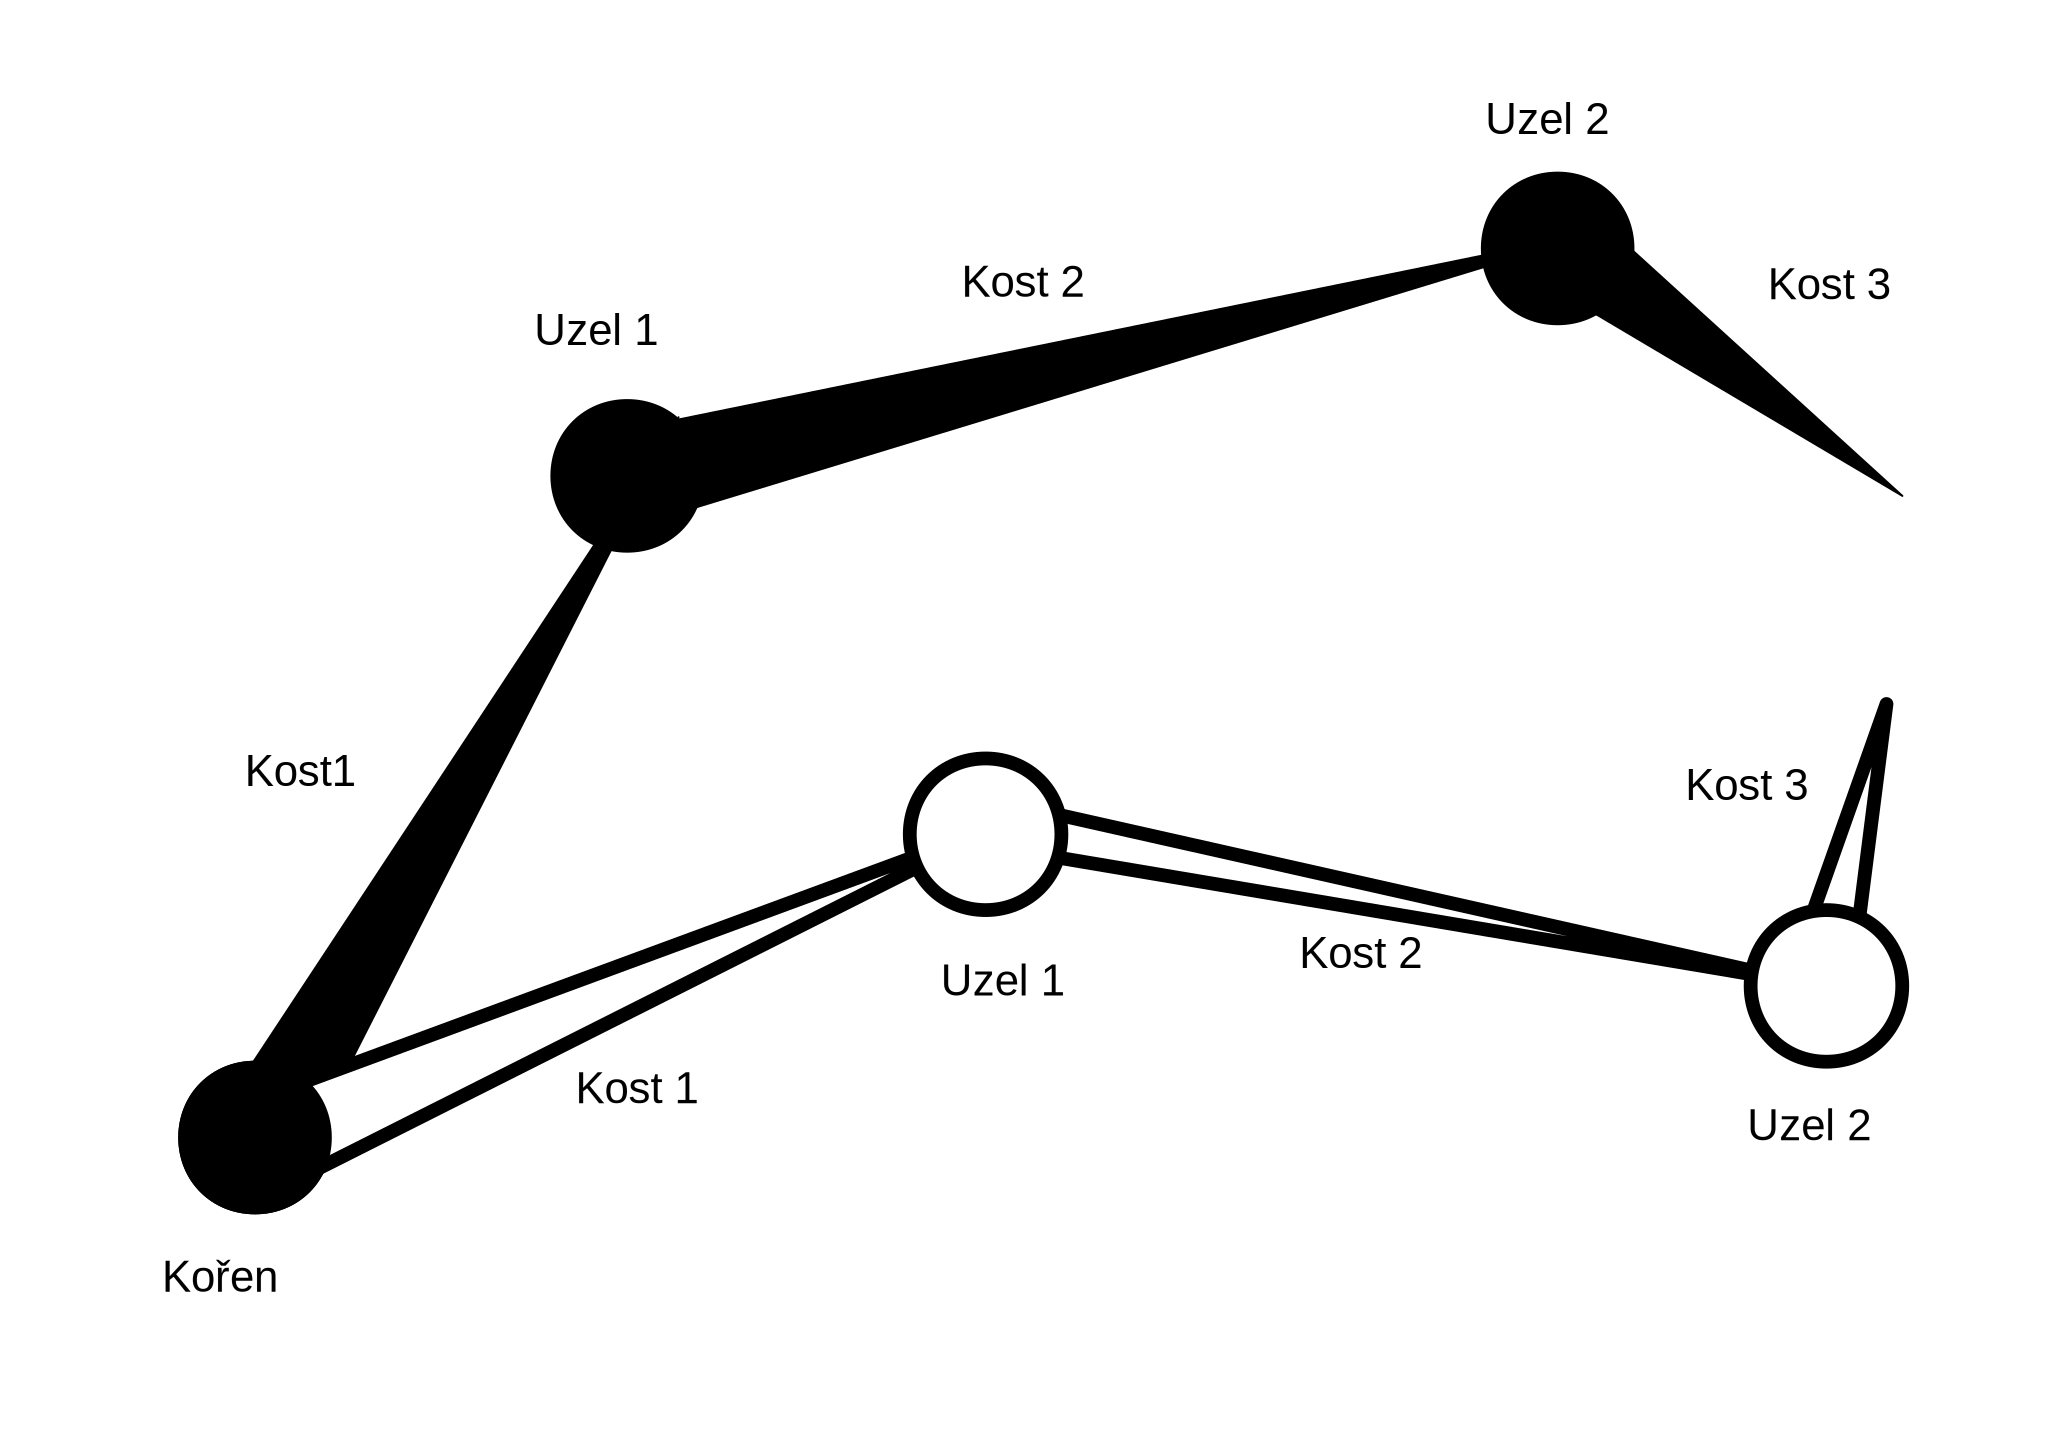
\includegraphics[scale=0.33 ]{obrazky-figures/skeletalAnimation}
\caption{Na obrázku vidíme náčrtek modelu s kostmi pro \emph{Skeleton animation} ve dvou různých časech (plná pro čas t, prázdná pro čas t+1).}\label{skeletalAnimation}
\end{center}\end{figure}
K výpočtu polohy vrcholu pro daný snímek se musí vypočítat kompletní transformační matice pro všechny kosti, kterými je vrchol ovlivněn. Matici kosti lze získat vynásobením všech matic uzlů od uzlu před danou kostí až ke kořeni, poté ještě násobeno transformační maticí kosti do souřadné soustavy bodů. Tyto matice po vynásobení příslušnými váhami a jejich sečtení, dávají výslednou transformační matici pro daný vrchol. Stačí samozřejmě vypočítat pro každou kost matici pouze jednou v daném snímku a pak při vykreslování vrcholů k ní jenom přistoupit. Matice pro uzly se mění v závislosti na čase animace. Ukládány jsou povětšinou pouze matice pro klíčové snímky. Je-li čas animace mezi dvěma klíčovými snímky, pak je potřeba k určení matice pro jeden uzel v čase t udělat vážený průměr matic z klíčového snímku před a po:
\begin{equation}\label{SAprumer}
M_t = \frac{M_{pred} \cdot (t - T_{po})}{M_{po} \cdot (T_{pred} - t)}
\end{equation}
Konkrétní implementace výpočtu a zpracování matic je uvedena v podkapitole \ref{SA-I}, kapitola Implementace. Vypočtou-li se všechny matice uzlů a z nich finální matice kostí, je transformační matice vrcholu dána vzorcem:
\begin{equation}\label{SAvzorec}
M_t = \sum_{0}^{n = pocet kosti} M_n \cdot vaha_n
\end{equation}
  
\section{Perlinův šum}
Perlinův šum byl navržen profsorem Kenem Perlinem v roce 1983 a v 1985 vydává text kde jej popisuje\cite{KP-old}. Tento šum se často používá k dosažení přirozeně náhodného jevu, jako jsou třeba letokruhy dřeva nebo skvrny na slunci. Používají se tři varianty Perlinova šumu a to 1D, 2D a 3D. 1D pro vytvoření linek, které vypadají jako kreslené rukou. 2D šum se používá například pro tvorbu 2D textur, také u výškových map náhodného terénu nebo pro zašumění normál textury pro dosažení dojmu hrbolatého povrchu. Trojrozměrná varianta šumu je asi nejzajímavější, protože je schopna generovat náhodné 3D objekty nebo prostory, například jako herní mapy s velkým počtem prvků.

Další z předností Perlinova šumu je, že profesor Perlin si jej nikdy nenechal patentovat. Díky tomu jej využívá spousta nekomerčních i komerčních aplikací. Dá se k němu dohledat spousta informací a není problém zjistit jak jej implementovat, neboť i sám profesor na svých stránkách\cite{KP-site} uvádí hned dvě implementace Perlinova šumu. 

V roce 2001 profesor Perlin vydal článek o \emph{Improved noise}\cite{KP-new}, kde popisuje nedostatky předchozí varianty šumu a cestu jak nedostatky odstranit. Já jsem se rozhodl ve své aplikace využívat \emph{Improved Noise}, který se od standardního Perlinova šumu liší jen v  gradientních vektorech a upravení funkce fade().
\begin{figure}
	\begin{center}
	\includegraphics[scale=0.25]{obrazky-figures/PN}
		\caption{Ukázka gratientních(g) a směrových(d) vektorů pro Perlinů šum}\label{aiAnimation}
\end{center}\end{figure}
Šum generuje náhodnou spojitou n-rozměrnou funkci. Hodnoty této funkce jsou počítány pomocí lineární interpolace a skalárního součinu gradientních a směrových vektorů. Vzorec \ref{PN-vz} ukazuje variantu pro 2D šum.
Kde \emph{lerp()} představuje funkci pro lineární interpolaci a funkce \emph{grad()}  provádí skalární součin směrového vektoru a gradientního vektoru vybraného permutační funkcí p(). V každém volání \emph{grad()} se použije jiný směrový vektor. 
\begin{equation}\label{PN-vz}
Noise(x,y) = lerp(v,lerp(u,grad(),grad()),lerp(u,grad(),grad()));
\end{equation}
\chapter{Návrh aplikace}\label{Navrh_aplikace}
Na začátku této kapitoly bude ujasněno co vše vlastně výsledná aplikace bude umět. Dále pak v jednotlivých podkapitolách budou tyto schopnosti podrobně popsány, zmíněné možné problémy, které z nich plynou a následně budou navrhnuta řešení. Bude-li více možností jak na danou vlastnost aplikace pohlížet, popřípadě jak s ní pracovat,  bude zdůvodněno proč bylo zvolené právě ono výsledné řešení. Pokud některá z vlastností aplikace bude řešena knihovnou třetích stran, bude v rámci popisu této schopnosti i navrhnuto její použití a práce s ní. V~rámci tohoto popisu bude i zdůvodněno proč je vlastně použita. Určitě budou tedy zmíněny knihovny jako je \emph{Assimp}\cite{assimp}  nebo \emph{Bullet physic library}\cite{bullet}, dále jen \emph{Bullet}. V kapitole \ref{implementace} Implementace  bude uveden výsledný diagram tříd vzniklý z tohoto návrhu.
\section{Obsah aplikace}
Cílem práce je vytvořit demo 3D hry, lukostřelecké střelnice. Demo bude tvořeno jen jednou scénou bez menu. Scéna bude obsahovat několik terčů a střeleckých pozic. Bude umožňovat pohyb avatárem ve vykresleném prostoru, tento hráč bude vybaven  lukem a několika šípy. Hráč vždy uvidí \emph{head-up display}, dále jen \emph{hud}, složený z počítadla bodů, ukazatele síly a směru větru, ukazatele zbylých šípů a zaměřovače. Pro šípy bude zajištěno fyzikální chování, ovlivnění silou a směrem větru. Scéna bude osvětlena pouze sluncem, dle herního času.
\subsection{Čeho všeho bude aplikace schopna}
\begin{itemize}
	\item Načítání a práce s modely a animacemi
	\item Fyzika letu a kolize objektů
	\item Osvětlení scény a stíny pro usnadnění odhadu vzdálenosti a realističnost
	\item Střídaní dne a noci
	\item Dostatečná náhrada slunce
	\item Vítr, plynulá změna jeho směru, poryvy, závětří
	\item Zvuková kulisa a zvuk výstřelu a dopadu šípu
\end{itemize}
\section{Načítání, ukládání modelů a jejich animací}

Modelem se rozumí skupina vrcholů (angl. \emph{mesh}). Aby aplikace mohla model vykreslit, musí být schopna jej načíst ze souboru a uložit si ho ve vhodné reprezentaci, a vědět kterou texturu má použít. K načtení bude použita knihovna \emph{Assimp}\cite{assimp}, aby bylo možno načítat více různých formátů. Model se bude ukládat jako pole vrcholů, kde vrchol bude představovat struktura. Ta bude obsahovat pozici vrcholu v souřadném systému modelu, uv koordináty, normálu, indexy a váhy kostí, na které vrchol bude navázán, více v sekci \ref{SA-I} o \emph{Skeleton animation}. V tomto poli bude každý vrchol pouze jednou, neboť aplikace bude vykreslovat metodou indexovaného kreslení.
    
Animace jsou načítány společně s modelem ze souboru, \emph{Assimp} je ukládá do dynamického seznamu struktur \emph{aiAnimation}. Každá z těchto struktur představuje jednu animaci modelu a vidět ji můžeme na obrázku \ref{aiAnimation}. 
\begin{figure}
	\begin{center}
		\includegraphics[scale=0.5]{obrazky-figures/aiAnimation}
		\caption{Část diagramu struktury knihovny \emph{Assimp}\cite{assimp} uchovávající informace o jedné animaci jednoho nebo více \emph{mesh} modelů.}\label{aiAnimation}
\end{center}\end{figure}

Vzhledem k tomu, že nad animací budou prováděny jen vyhledávací a čtecí operace, je toto uspořádání dostačující. Pokud by ovšem vyhledávací a výpočetní funkce byly přidány do stejné třídy, kde už jsou metody pro práci s modelem, tak by se tato třída stala velice přetíženou a těžko odladitelnou. Proto bude vhodné zabalit tuto strukturu do vlastní třídy, obohatit ji o potřebné metody a ve třídě pro model zpřístupnit jen výsledné transformační matice jednotlivých kostí.

 Modely se vyskytují ve spoustě různých formátech a variacích, rozhodl jsem se pracovat pouze se dvěma formáty:
\begin{itemize}
	\item \emph{Wavefront} od \emph{Wavefront Technologies} s příponou \emph{obj} pro modely bez animací
	\item \emph{COLLADA} od \emph{Sony Computer Entertainment} s příponou \emph{dae} pro modely s animacemi.
\end{itemize}

Ke čtení modelů je sice použit \emph{Assimp::Importer}, který je schopen číst širokou škálu formátů, ovšem aplikace je odzkoušena pouze na těchto dvou formátech. Při jiných formátech by potom mohlo dojít k problému při přiřazování do třídy \emph{Model} viz diagram tříd \ref{ClassDia}.
\section{Fyzika letu a kolize objektů}
V této části bude navrženo řešení výpočtu pohybu těles v gravitačním poli a výpočet projevu sil, jako například výstřel šípu. S tímto chováním i úzce souvisí kolize mezi objekty.

Fyzikální popis těchto jevů a chování je relativně složitou záležitostí a vytvoření dostatečně rychlé implementace těchto jevů by výrazně přesáhl rámec této práce, pro to jsem se rozhodl použít externí knihovnu \emph{Bullet physic engine}\cite{bullet}. Tato knihovna poskytuje i možnost řešení kolizí a jejich zachytávání.  

Ovšem nepracuje přímo s modely co jsou vykreslovány, ale s vlastními objekty typu \emph{btCollisionObject}, proto je potřeba vytvořit vazbu mezi vykreslovanou scénou a scénou, se kterou pracuje \emph{Bullet}, povětšinou \emph{btDiscreteDynamicWorld}. Tato vazba musí být obou směrná neboť při každém snímku se musí aktualizovat poloha vykreslovacích modelů polohou jejich fyzikálních ekvivalentů. A naopak \emph{Bullet} vrací kolize jako pole dvojic \emph{btCollisionObject} kdy pro každý objekt z tohoto pole se musí zavolat funkce pro reakci na kolizi. 

    
\section{Osvětlení a stíny}
Scénu bude osvětlovat pouze jeden zdroj směrového světla představující slunce, měsíc svítit nebude, za použití Phongova osvětlovacího modelu. Jeho poloha a intenzita se bude měnit dle herní denní doby.   
Stíny budou vypočteny a vykresleny metodou \emph{shadow maping }jenž je popsána v kapitole \ref{shadowMap}. Protože aplikace bude mít jen jeden  zdroj směrového světla, je tato metoda vhodná, právě díky své rychlosti a stačí také vytvořit pouze jednu mapu. Tato mapa se bude přepočítávat pro každý snímek zvlášť, může se tedy vždy namapovat na scénu tak, aby měla co nejmenší přesah přes plošné promítnutí tělesa vymezeného pohledem kamery a zdrojem světla. Tento způsob namapování umožňuje pracovat s menší texturou, což urychlí její výpočet a zabírá tak méně paměti, nebo pracuje se stejně velkou texturou, díky čemuž se získají lepší detaily. Poloha tohoto zdroje světla bude navázána na příslušný objekt, který jej bude představovat. Společně s tímto objektem bude zdroj putovat po obloze a díky \emph{diffusní} části světla se na základě úhlu mezi zdrojem a horizontem bude měnit i intenzita osvětlení. 
\section{Střídání dne a noci}\label{dayNight}
Na \emph{skybox} se budou mapovat celkem dvě textury pro denní a noční oblohu. Střídání dne a noci je způsobeno změnou poměru míchání noční a denní textury pro jednotlivé fragmenty.

    \begin{figure}
    	\begin{center}
    		\includegraphics[scale=0.35]{obrazky-figures/dayOnight}
    		\caption{Graf střídání denní a noční oblohy, kdy poloha osy fragmentu vůči ose 0 a 1 určuje poměr míchání textur pro tento fragment. Osy 0 a 1 na základě herního času rotují a dělí den na 8 částí. }\label{dayOnight}
    \end{center}\end{figure}

Poměr pro každý fragment je dán úhlem mezi jeho osou (polopřímka ze středu přes něj) a osami 1 a 0, jak je vidět na obrázku \ref{dayOnight}. Pokud se fragment nachází ve stejném kvadrantu jako osa 0, je poměr vypočítán na základě jeho úhlu. Je-li úhel 45\degree,  je poměr míchání 0:1 v neprospěch aktuálního cyklu, naopak pro -45\degree~je poměr 1:0 pro aktuální cyklus. Mezi těmito hodnotami je potom nepřímá úměra. Ve zbylých třech kvadrantech je poměr vždy buď 1:0 nebo 0:1, odvíjí se od toho, která čtvrtina  denního/nočního cyklu je:
\begin{itemize}
	\item kvadrant u osy 1:
	\begin{itemize}
		\item[-] pro 1 - 3 část cyklu 0:1
		\item[-] pro 4 část cyklu 1:0 
	\end{itemize}
	\item kvadrant naproti ose 0:
		\begin{itemize}
		\item[-] pro 1 a 2 část cyklu 0:1
		\item[-] pro 3 a 4 část cyklu 1:0
	\end{itemize} 
	\item kvadrant naproti ose 1:
		\begin{itemize}
		\item[-] pro 1 část cyklu 0:1
		\item[-] pro 2 - 4 část cyklu 1:0 
	\end{itemize}
\end{itemize}
Celý den má tedy 8 částí, 4 denní a 4 noční, což trvá dvě otočení os o 360\degree. Aplikace při spuštění začíná v čase nula, tedy úsvitem nového dne.
\section{Slunce a měsíc} 
Slunce a měsíc se realizují pomocí plochých modelů rotujících kolem středu \emph{skyboxu}. Doba oběhu musí trvat celý den, tedy dvě otočení os \emph{skyboxu}. V rámci třídy pro slunce a měsíc se bude řešit i změna směru světla příslušného objektu. Pro správný pohyb se musí zajistit dvě věci. Za prvé správné natočení plochy objektu, aby nebyl vidět jako elipsa či jako pouhá čára. A za druhé uchování vzdálenosti od středu \emph{skyboxu}, potažmo avatara. Dosáhne se toho pomocí vektoru $\vec{a}$ mezi středem a objektem a rotací $\vec{a}$ i objektu kolem stejné osy (vyjádřená stejným předpisem, počítána vždy v relativní soustavě objektu nebo globální soustavě v případě $\vec{a}$). Poloha objektu se potom vždy nastaví podle vektoru $\vec{a}$ posunutého do aktuálního středu \emph{skyboxu}.
\section{Vítr}
Vítr je na vykreslování relativně jednoduchý jev, není totiž vidět, na druhou stranu má spoustu viditelných projevů. Prozatím se bude práce zabývat pouze působením větru na šíp za letu.
Vítr bude mít globální sílu a směr, který se bude v čase měnit. Takto by byl vítr všude stejný, jenže vítr se mění. Vítr je ale možno zastavit, vznikají tak závětří, jinde pofukuje více, či méně, tamhle trochu jiným směrem. Aby se dalo dosáhnout tohoto chování alespoň do jisté míry realističnosti, je potřeba určit závětrná místa, větrné stíny, a pro každý bod vypočíst drobnou odchylku směru a síly, jak je znázorněno v obrázku \ref{windmap}.

\begin{figure}
	\begin{center}
		\includegraphics[scale=0.5]{obrazky-figures/windMap}
		\caption{Větrná mapa výsledné aplikace. Šipky znázorňují směr a velikost větru. Za~oběma čtverci je možno vidět větrné stíny s výrazně nižší intenzitou větru.}\label{windmap}
\end{center}\end{figure}
K výpočtu větrných stínů se dá použít téměř jakákoliv osvětlovací metoda, protože vítr se v podstatě v~ničem neliší od světla. Stále to jsou paprsky/proudy a pouze jejich projevy se liší, místo osvětlení fragmentu posunou objekt, na který dopadly. Já jsem se rozhodl použít metodu \emph{shadow maping} a znovu využít již nutně implementované funkce pro výpočet stínů osvětlení. Tímto postupem lze získat větrné stíny, ovšem síla a směr větru se měnit nebude. Proto výsledná mapa ze \emph{shadow mapingu} bude zašuměna, například již zmíněným \emph{Perlinovým šumem}. Pro tuto bakalářskou práci připadají dvě možnosti. Buď zašumit vždy celou mapu, nebo pouze aktuálně čtený bod. Vzhledem k tomu, že vítr bude ovlivňovat pouze několik těles a pro každé těleso se bude číst jen jeden bod z mapy (důvod proč jen jeden bod bude vysvětlen dále). Proto bude rychlejší na výpočet použít šum vždy až při čtení bodu.

Ještě zbývá vyřešit, jak se bude vítr projevovat. K tomu lze přistoupit dvěma způsoby: jednodušším a méně reálným nebo složitým a reálnějším. Jednoduší znamená, že se vítr bude projevovat jako pouhá směrová síla, bez ohledu na dopadovou plochu tělesa. Složitý přístup znamená vypočítat dopadovou plochu a z ní odvodit výslednou sílu větru. K~zjištění dopadové plochy by bylo ovšem potřeba každý fragment tělesa otestovat na jeho polohu v mapě, jestli je ve stínu nebo ne. Pokud by se tento test prováděl na CPU, došlo by k~výraznému zpomalení aplikace, na GPU by k~zpomalení nedocházelo, a v ničem by se to nelišilo od vykreslování stínů, ovšem standardní knihovny pro práci s GPU neumožňují přesun dat z GPU zpět do CPU. Pokud by šlo o simulátor plachetnice, tak by se určitě muselo jít složitější cestou, ale tím, že je v rámci výsledné práce tvořena lukostřelecká střelnice, vítr bude primárně ovlivňovat šípy, které mají relativně malou plochu a dalo by se říci, že stejnou ze všech stran, bude tedy dostačující pouze jednoduchá cesta, která byla popsána výše. Z toho také vyplývá proč se bude vždy číst jen jeden bod mapy pro těleso a stačí tím pádem aplikovat šum až při čtení bodu.

\section{Zvuková kulisa a zvuk výstřelu a dopadu šípu}
Pro výsledný efekt by bylo poněkud nezvyklé, kdyby se během hry neozývaly žádné zvuky, tento drobný detail by způsobil poloviční zážitek, i kdyby by byla hra sebelepší. Ovšem podobně jako v případě působení sil i šíření zvuku v 3D prostoru, to není zcela triviální záležitostí. Za prvé, pokud je třeba rozpoznat zdroj zvuku ve scéně, je potřeba pracovat s~různou úrovní hlasitosti pro každou stranu. A za druhé přehrávaný zvuk musí běžet ve vlastním vlákně, jinak by pozastavil vlastní aplikaci, do doby než by skončilo jeho přehrávání. Z těchto dvou důvodů jsem zvolil externí knihovnu \emph{IrrKlang}\cite{irrKlang}, která obě požadované vlastnosti poskytuje skrze jednu funkci. Vývojáři této knihovny se opravdu řídili heslem v~jednoduchosti je síla a pro většinu případů stačí metoda \emph{play3D(paht,option)}, kde \emph{option} určuje, zda-li zvuk běží ve smyčce nebo ne.  
\chapter{Implementace}\label{implementace}
V první části této kapitoly bude popsán diagram tříd výsledné aplikace, v diagramu jsou uvedeny pouze třídy, jenž jsou nějak zajímavé nebo důležité. Třídy, které slouží jen k zapouzdření a zpřehlednění kódu budou vynechány. V druhé části této kapitoly budou podrobně popsány zajímavé problémy, na které jsem při implementaci narazil.  
\section{Diagram Tříd}
Na obrázku \ref{ClassDia} je zjednodušený diagram tříd výsledné aplikace. Výsledná Aplikace je složena ze tří hlavních částí:
\begin{enumerate}
	\item Třída \emph{Scene}, která zapouzdřuje celou aplikaci.
	\item Třída \emph{BulletWorld}, přes kterou je řešena veškerá fyzika.
	\item Třída \emph{Model}, která je výchozí třídou pro většinu prvků ve scéně.
\end{enumerate} 
Dále pak má aplikace  mnoho dalších tříd, jako třídy pro hud nebo pro práci s animacemi či zvukem, mezi zajímavější pak patří třídy \emph{Skybox} a \emph{SunMoon}, které mají na starosti celé střídání dne a noci a pohyb zdrojů světla. 
\begin{figure}
	\begin{center}
		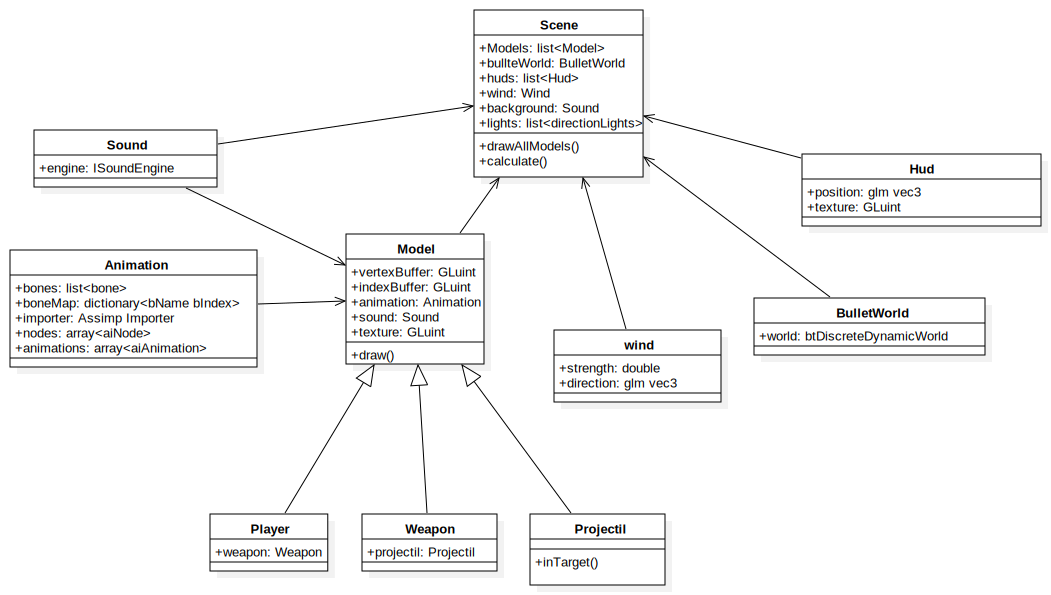
\includegraphics[scale=0.5]{obrazky-figures/ClassDia}
		\caption{Zjednodušený diagram tříd výsledné implementace}\label{ClassDia}
\end{center}\end{figure}


\subsection{Třída \emph{Scene}}
Třída \emph{Scene} je ústřední třídou, z níž se přistupuje do třídy \emph{BulletWorld} pro detekci kolizí a změny poloh modelů, na základě působení sil. Zde se také řeší jednotlivé kroky vykreslování, jako vykreslení do \emph{wind mapy, shadow mapy} a výsledné vykreslení.

Třída \emph{Scene} tím pádem obsahuje převážně funkce pro nastavení objektů, jejich vkládání a případné nastavení propojení mezi objekty, které spolu nějak komunikují (např.: zbraň a projektil nebo objekt a jeho fyzikální představitel). Většina chování objektů je v jejich vlastní režii, třída \emph{Scene} volá jen funkce pro jejich nastavení při vzniku a během cyklu už pouze vykreslovací funkce.  

Tato třída ještě obsahuje slovníky načtených modelů a textur. Slovník pro modely má tvar \emph{<cestaKsouboru,ImportModel>}. Při načítání souboru se zkontroluje, zdali již není ve~slovníku, jestliže je, použije se příslušný záznam. Není-li tomu tak, tak se soubor načte a zpracuje do třídy \emph{ImportModel} a vrátí se opět záznam ze slovníku. U textur to probíhá podobně jen místo třídy \emph{ImportModel} se použije přímo adresa textury na GPU.
\subsection{Třída \emph{BulletWorld}}
\emph{BulletWorld} provádí operace nad \emph{btDiscreateDynamicWorld} z knihovny \emph{Bullet}\cite{bullet}, tedy inicializační a úklidovou (v rámci destruktoru třídy) metodu pro \emph{btDiscreateDynamicWorld}, dále metody pro několik variant vkládání \emph{btCollisionObject}
a nejdůležitější metoda je \emph{calculate()}, která zjistí a vrátí list aktuálních kolizí. Tato metoda je využita ve třídě \emph{Scene}, která dále zajistí zavolání metody \emph{hitted(Model*)} pro každý z kolizních objektů, kdy parametr této funkce je vždy objekt, se kterým došlo ke kolizi. 

U této části je problém, protože není-li volání této funkce o stejné frekvenci jako tiky v \emph{Bullet engine}, tak se některé \uv{stejné kolize} zachytí několikrát. Ony to nejsou stejné kolize, ale dojde-li ke střetu dvou objektů, tak doba jejich dotyku není nekonečně malá a může přesáhnout do několika tiků v \emph{btDiscreteDynamicWorld}, což vytvoří několik záznamů o~kolizi.
V důsledku tohoto jevu se v seznamu kolizí některé kolize vyskytují několikrát, k~ošetření dochází ve třídě \emph{ Scene}. Všechny kolize dané dvojice se ze seznamu vymažou, když třída \emph{Scene} zavolá metodu \emph{hitted(Model*)} pro daný pár objektů.
\subsection{Třída \emph{Model} a její potomci}
Téměř všechny objekty ve scéně dědí od této třídy. Jediné které od ní nedědí je třída \emph{Wind} a třída pro prvky hud. V třídě \emph{Model} jsou tedy implementace základního vykreslování a obecná práce s polohou, vytváření \emph{bufferů}, výchozí implementace metody \emph{hitted(Model*)}. Většina potomků tyto metody dědí nezměněné.

Třídy \emph{Weapon a Projectil} přepisují metodu \emph{getPosition()}. Poloha \emph{Weapon} se určuje na základě polohy přiřazené třídy \emph{Player}. U třídy \emph{Projectil} je to komplikovanější, neboť má tři stádia života, a to ve zbrani, v letu a v zabodnutí. V případě stadií ve zbrani a zabodnutí je poloha určována na základě modelu, ve kterém je (zbraň nebo objekt, ve kterém je zabodnut). Během letu se jeho poloha odvozuje jako u ostatních modelů, tedy od polohy jeho fyzikálního ekvivalentu. Více o vztahu těchto tří tříd bude řečeno v podkapitole \ref{PWP}
\subsection{Třídy \emph{Skybox} a \emph{SunMoon}}
Tyto třídy sice také dědí od třídy \emph{Model}, jako jediné ale v podstatě dědí pouze rozhraní neboť, tři hlavní metody \emph{draw()}, \emph{drawToShadowMap()} a \emph{getPosition()}, celé přepisují a ani nevlastní svůj fyzikální ekvivalent v \emph{btDiscreteDynamicWorld}. \emph{Skybox} má i vlastní speciální sadu \emph{shaderů}.

Změnu denní a noční oblohy řídí funkce \emph{calcAxis()}, která přepočítává rotace os a také na základě jejich úhlů vůči osám x a y určuje fázi denního/nočního cyklu. Ty jsou vysvětleny v kapitole \ref{dayNight}. Původně se fáze cyklu měly měnit pouze na základě času, ale v tom případě by musely všechny části trvat stejně, což sice odpovídá realitě, ale nevypadá to věrohodně. Rozednívání je moc pomalé a stmívání také, jako více věrohodná  se ukázala varianta, kdy je přechod mezi druhou a třetí  fází denního i nočního cyklu, obrázek \ref{dayOnight}, trojnásobně zrychlen a zde ušetřený čas je rozložen mezi zbylé tři přechody. Úroveň tohoto zrychlení byla zjištěna empiricky, metodou pokus omyl. Tahle varianta vytváří i lepší koordinaci mezi stavem oblohy a pohybem slunce, tedy když slunce vyjde, tak se rychle rozední a pak slunce pomalu putuje po obloze během dne. Jakmile slunce zapadne, tak se rychle setmí. Při stejné rychlosti všech fází by se slunce, mělo-li stejnou dobu oběhu jako byla délka dne, drželo by se ve stejné části oblohy. Pokud ale mělo dobu oběhu delší, tak by se slunce zpožďovalo o~proti rozednění v následujících dnech. 

\emph{Skybox} využívá jiný \emph{shader}, jak již bylo zmíněno, kvůli způsobu určování poměrů pro \emph{multiTexturing}. Kvůli výpočtu poměru je potřeba, aby \emph{shader} vždy věděl, co je za část dne a znal osy. Na druhou stranu vůbec nepracuje se světly, proto má \emph{skybox} i jinou \emph{draw()} metodu. \emph{Skybox} i \emph{SunMoon} se do \emph{shadow mapy} vůbec nevykreslují, proto nad nimi vůbec metoda \emph{DrawToShadowMap()} není volána.

\emph{SunMoon} je třída pro nebeská pohyblivá tělesa, má metody pro nastavení doby oběhu, sklonu osy vůči povrchu, posun času východu a nezačíná tak na horizontu. Podobně jako Skybox i třída SunMoon používá vlastní, v tomto případě výrazně jednoduší shader, protože nad ní se neprovádí ani  výpočet stínů a osvětlení ani \emph{Skeleton animation}. Takže by bylo zbytečné mít tak rozsáhlí shader. Z toho opět plyne jiná \emph{draw()} metoda.        
\subsection{Třída \emph{Hud}}   
\emph{Hud} je výchozí třídou pro všechny prvky \emph{head-up diplay}. Zajišťuje namapování příslušných textur na určené místo na obrazovce. Potomci této třídy  jsou třídy na zobrazování stavu toulce (třída \emph{ArrowStack}), zaměřovač (\emph{CrossHair}) a univerzální třída na výpis řetězce (\emph{HitsHud}).

\emph{ArrowStack} zobrazuje pouze na obdélník, jenž je mu nastaven. Nastavená oblast obrazovky je rozdělena horizontálně na tolik oblastí, na kolik je nastaven atribut \emph{initialCount}, zde pak zobrazí tolik textur, kolik je hodnota \emph{countOfArrow}, každou texturu na jednu oblast. Díky tomu je znovu použitelný na n-násobné zobrazování jakékoliv textury v HUD.
 
\emph{HitsHud} zobrazuje řetězec znaků pomocí textury znakové tabulky. V nastavení se určí velikost jednoho znaku a počátek řetězce. Poté se při výpisu pro každý znak spočítá obdélníček a uv souřadnice v textuře na základě \emph{ascii} hodnoty, modulo počtem sloupců textury se získá x souřadnici a děleno počtem řádků y souřadnici. Výpočtem byl získán buď levý dolní nebo levý horní roh. Který z těchto rohů byl vypočten se odvíjí od orientace textury. Tato třída je počítána na orientaci, kdy bod [0,0] leží v levém dolním rohu a znak s~hodnotou~0~je v levém horním.  
\subsection{Třída \emph{Wind}}
V režii této třídy je zajištění \emph{wind map} a čtení na základě souřadnic pomocí metody \emph{getLocalWind(glm::vec3)}. Metoda vrací proměnou typu \emph{glm::vec3} vypočítanou vzorcem \ref{vitr}. Jinak je tato třída dosti podobná implementaci stínů. Pro vykreslování do \emph{wind map} se používá speciální metoda ve třídě \emph{Scene}, ale jde jen o nastavení parametrů pro zápis, jinak by se dala použít stejná metoda jako pro zakreslování do \emph{shadow map}. V obou těchto metodách se volá pro jednotlivé modely ta stejná metoda, \emph{drawToShadowBuffer()}. 
\begin{equation}\label{vitr}
\vec{v} = \overrightarrow{direction} \cdot PerlinNosice(x,y) \cdot strength \cdot shadow
\end{equation}
Ve vzorci \ref{vitr}:
\begin{itemize}
	\item direction = směr větru
	\item strength = síla větru
	\item \emph{PerlinNoise(x,y)} způsobí zašumění směru a síly, pro náhodnější jev
	\item shadow je koeficient pro závětří, 1 pro volný prostor a 0,5 pro závětří
\end{itemize}
\subsection{Třída \emph{Animation}}
Pokud je při načítání modelu zjištěno, že obsahuje animaci, tak je vytvořena třída \emph{Animation} a ta je pak navázána na vznikající ImportModel. V této třídě jsou obsaženy kosti a uzly pro příslušnou animaci a odkaz na \emph{aiAnimation} obsahuje vlastní animaci. Kosti jsou uloženy jako vektor mých struktur \emph{Bone}, ale pole uzlů a animace využívá struktury \emph{aiNode} a \emph{aiAnimation}. Na obrázku \ref{aiAnimation} je vidět právě \emph{aiNodeAnim}, která slouží jako mapovací třída mezi animací a polem uzlů. V případě rozšíření aplikace o možnost vytvořit více animací pro jeden model, budou se úpravy týkat pouze třídy \emph{Animation}, více v sekci 5.3 Možnosti rozšíření. Prozatím je ale počítáno pouze s jednou animací.
zšíření, zatím počítáno pouze s jednou animací. 
\subsection{Třída \emph{Sound}}
Třída \emph{Sound} je určená pro práci s knihovnou \emph{IrrKlang}\cite{irrKlang}. Hlavním důvodem vzniku této třídy je zpřehlednění a zapouzdření kódu, tak aby \emph{Model} při určité situaci mohl zavolat metodu \emph{play3D(path)} a o více se nemusel starat. Knihovna \emph{IrrKlang} umožňuje asynchronní přehrávaní, tedy přehrávání zvuků nezpožďuje scénu ani nepozastavuje výpočty aplikace.

 Všechny instance této třídy by měly pracovat s jedinou instancí \emph{ISoundEngine} z knihovny \emph{IrrKlang}, která je inicializována v rámci třídy \emph{Scene} a modelům ve scéně je pak předána pouze jako parametr. Důvod je ten, že pro každou instanci \emph{ISoundEnginu} se musí nastavit poloha posluchače a většina modelů nemá přístup k poloze hráče. 
\section{Zajímavé nebo problémové části implementace}
Tato podkapitola podrobněji popíše implementaci míst, kde se musel řešit nějaký implementační problém nebo bylo použito netradičního, či zajímavého řešení.

Popsáno bude řešení vztahu mezi hráčem, zbraní a projektilem,  práce se \emph{shadery} (kolik jich je použito, jak se předávají mezi instancemi\dots), nakonec \emph{Skeleton animation}. 
\subsection{\emph{Player}, \emph{Weapon} a \emph{Projectil}}\label{PWP}
Při implementaci této části došlo k problému jak tyto tři třídy provázat, varianta A nebo B viz obrázek \ref{PWPpicture}. Varianta A umožňuje řídit vše přes hráče, tedy od nejstálejší třídy (hráč se nebude pravděpodobně měnit nikdy, zatímco zbraň se občas změnit může a projektil se bude měnit po každém výstřelu). Tato varianta je příjemná pro řízení výstřelu a nabití, ovšem pro vykreslování má jednu nepříjemnou vlastnost, a to, že se musí začít od hráče a ten musí aktualizovat polohu zbraně a ta projektilu, takže je-li pořadí vykreslování opačné, mají zbraň i projektil vždy polohu o snímek zpět. Ve variantě B si o aktualizaci polohy vždy nižší prvek může říct a tím pádem nezáleží na pořadí. Ovšem při této variantě by se musel uchovávat místo hráče projektil, který se po každém výstřelu mění, také by bylo celkem komplikované vystřelit a znovu nabít, nemluvě o případě, že dojdou šípy.

Ideální varianta by byla kruhová závislost ovšem C\texttt{++} tuto variantu není schopno zkompilovat. Ale pokud se v jednom směru použije konkrétní třída (\emph{Player, Weapon, Projectil}) a ve druhém směru rodičovská třída \emph{Model}, tak tuto obousměrnou závislost lze provést. A jeden směr tak bude sloužit k výstřelu, zatímco druhý bude sloužit k získání pozice.
    \begin{figure}
	\begin{center}
		\includegraphics[scale = 0.6]{obrazky-figures/PWP}
		\caption{Varianty provázání \emph{Player}, \emph{Weapon} a \emph{Projectil}. Šipky naznačují, které třída bud obsahovat ukazatel na druhou třídu.}\label{PWPpicture}
\end{center}\end{figure}
\subsection{Shadery}
\emph{Shadery} jsou programy běžící na GPU a probíhají v nich vykreslovací výpočty pro jednotlivé vrcholy a fragmenty (\emph{vertex} a \emph{fragment shader}). Protože některé modely v jistých situacích vyžadují jiné výpočty, než jindy obsahuje aplikace hned několik sad \emph{shaderů} (např.: pro vykreslování do \emph{shadow mapy}, bežné vykreslení scény, \emph{skybox}, \dots). Všechny jsou k nalezení na přiloženém DVD ve složce /src/shaders. 

 Možností je pro každý model načíst potřebné \emph{shadery}, zkompilovat je a používat, ale to by zabíralo hodně paměti a zpomalovalo aplikaci. A většina objektů potřebuje ty stejné \emph{shadery}, téměř všichni potomci třídy \emph{Model} používají \emph{shadowMap.v/fs} a \emph{diffuseLight.v/fs}. Tento problém jsem vyřešil tak, že tyto dva \emph{shadery} načte a uchovává třída \emph{Scene} a modelům předává jen jejich adresu. Když následně bylo potřeba přidat \emph{shadery} pro prvky hud vznikl problém, pokud by se opět přidaly do třídy \emph{Scene}, stala by se tato třída velice špatně čitelnou a vznikla by zde spousta podobných a zaměnitelných atributů. Proto pro všechny instance třídy \emph{Hud} a jejich potomků je \emph{shader} jako statický atribut. Takže první vzniklá instance jej načte a zkompiluje nebo se zavolá příslušná statická metoda, ostatní už jen přistupují k tomuto atributu. 
 
 Varianta se statickým atributem je pracovně mnohem příjemnější, protože model pro své vykreslení potřebuje relativně hodně proměných typu \emph{uniform} jejiž adresu si je třeba najít a pamatovat. To se může udělat v rámci funkce, kdy model dostane adresu \emph{shaderů} \emph{setShader()}, ale tím vznikne několik míst, kde se napevno nastavuje konstanta (jméno proměnné v \emph{shaderu}), což by při úpravách kódu mohlo způsobit nepříjemnosti. Na druhou stranu, předají-li se jí tyto adresy jako parametry, vznikne funkce asi s 9 parametry, což není vůbec praktické. V aplikaci je to pro zatím řešeno tak, že část se nastavuje v \emph{setShader()} a část se předá parametrem. A tady přichází na scénu statické atributy. Pokud se totiž použije tato varianta, vše se může tím pádem nastavit v metodě \emph{setShader()} a to pouze jednou a na jednom místě v kódu. 

\subsection{Implementace Skeletal Animation}\label{SA-I}
Tato podkapitola rozebere způsob vyhledávání záznamů ve struktuře \emph{aiAnimaton} a jejich následující zpracování. Nejdříve bude vysvětlena část probíhající na CPU, na GPU probíhá opravdu jednoduchý děj, jenž bude popsán na konci.

Kosti jsou uloženy ve vektoru mnou vytvořených struktur \emph{Bone}, struktura vždy obsahuje matici odsazení a naposledy vypočítanou finální matici. Pro vykreslení objektu s animací v~čase t potřebujeme znát finální matice kostí pro čas t. Na výpočet těchto matic je potřeba projít strom \emph{aiNode} a pole \emph{aiAnimation}, jenž jsou uloženy ve třídě \emph{Animation}.
    \begin{figure}
	\begin{center}
		\includegraphics[scale = 0.5]{obrazky-figures/aiATree}
		\caption{Graf konkrétní instance struktur \emph{aiScene}. Jsou vidět všechny tři podstruktury, ve kterých jsou uložena data potřebné k realizaci animace. Přerušované čáry spojují ekvivalentní objekty.}\label{aiAtree}
\end{center}\end{figure}

\emph{Assimp} ukládá načtený soubor do struktury aiScen, jejíž příklad je vidět na obrázku \ref{aiAtree}. Vektor kostí z \emph{aiMesh}, odkaz na vrchol stromu \emph{aiNodes} z \emph{aiScene} i odkaz na strukturu \emph{aiAnimation} z \emph{aiScene} jsou přeneseny do třídy Animation. K získání finálních matic pro animaci v čase t je potřeba projít strom uzlů. Pro každý uzel je potřeba vyčíst matici z pole struktur \emph{aiNodeAnim} v \emph{aiAnimation} a vynásobit s maticemi všech předků a předat kosti.
  
Rozhodl jsem se strom procházet rekurzivně a algoritmus vypadá zhruba takto (pseudokód):  
\lstset{frame = single, language=C++, framexleftmargin=15pt,label="Algoritmus"}

\begin{lstlisting}[caption=Algoritmus pro projití stromu uzlů]
void updateNode(Node *n, Matrix4x4 m, time t){
	Matrix4x4 nodeM = getMatrixfromAiAnimation(n->name,t);
	Matrix4x4 toGlobal = inverse(m*nodeM);
	if(findBone(n->name)){
		Bone * bone = getBone(n->name);
		bone->final = toGloba * bone->offset;
	}
	for each(Node child in n->child){
		updateNode(child, toGlobal)
	}
}
\end{lstlisting}
\vspace{10pt}
Pro získání matice aktuálního uzlu je potřeba v poli \emph{mChanels} v \emph{aiAnimation} vyhledat záznam se stejným jménem jako má uzel. Jestliže byl nalezen správný \emph{aiNodeAnim}, pak je potřeba z něj vyčíst vektor posunutí, kvaternion rotace a vektor zvětšení. Pro výpočet těchto prvků pro čas mezi klíčovými snímky se použije vzorec \ref{SAprumer} vysvětlený v kapitole \ref{SA}. Z těchto dvou vektorů a kvaternionu bude sestavena hledaná transformační matice.

Na GPU probíhá pouze násobení matic váhami a jejich sečtení. Tyto operace se provádí v rámci \emph{vertex shaderů}. Výsledná matice je použita spolu s \emph{model view projction} maticí a souřadnicemi bodu. Jak je vidět v následujícím úryvku kódu ze souboru \emph{diffuseLight.vs}.
\lstset{basicstyle=\footnotesize, frame = single, language=C++, framexleftmargin=15pt,label="Algoritmus"}
\lstinputlisting[language=c++, firstline=20, lastline=30,caption=Ukázka práce \emph{skeletal animation} ve \emph{vertex} \emph{shaderu}.]{diffuseLight.vs}\label{SA-shader}

\chapter{Shodnocení náročnosti a efektivnosti implementace}
První část této kapitoly se bude zabývat schopnostmi a výkonem aplikace, dále její chování v určitých situacích, jako je načítání nového objektu či jiná nečekaná událost, třeba jeho nenalezení. Při nepříznivé reakci budou navrhnuty možné příčiny a následné opravy.

 Druhá část se bude věnovat možnými rozšířeními aplikace pro lepší výkon a vzhled. Půjde spíše o myšlenky a návrhy než rozbor konkrétní implementace nebo teorie. 
\section{Náročnost a výkon}
Tato podkapitola se bude zabývat jak se mění náročnost na paměť a počet snímků za sekundu během a po:
\begin{itemize}
\item vložení mnoha stejných modelů
\item vložení hodně různých modelů
\item vložení několika středních modelů	
\end{itemize}
\subsection{Vložení mnohokrát jednoho modelu}
Pokud se opakovaně vloží jeden a ten samý model několikrát, mohlo by nastat dočasné zpomalení aplikace a zároveň dojde ke zvýšení zabrané paměti při vložení toho prvního, ale při každém dalším by se již neměla zvednout paměť ani klesnout framerate.

Tuto vlastnost otestuji se dvěma modely. V každém snímku vloží novou instanci objektu \emph{sphere.obj} nebo \emph{cube.obj} až do celkového počtu 100. U krychlí by se předpoklad měl vyplnit určitě, ale koule jsou již relativně složitý útvar (myšleno počtem vrcholů).
\begin{figure}[!tbp]
	\centering
	\begin{minipage}[b]{0.4\textwidth}
		\includegraphics[width=\textwidth]{obrazky-figures/19}
		\caption{Během vkládání koulí}
	\end{minipage}
	\hfill
	\begin{minipage}[b]{0.4\textwidth}
		\includegraphics[width=\textwidth]{obrazky-figures/20}
		\caption{Po ustálení koulí}
	\end{minipage}
\end{figure}

Výsledek pro krychle je: 
\begin{enumerate}
	\item K navýšení paměti opravdu nedošlo. Tedy optimalizace s třídou \emph{ImportModel} funguje jak mám.
	\item Ovšem u počtu snímků za sekundu došlo k výraznému poklesu až do doby kdy se pozice krychlí neustálili. Důvodem tohoto jevu je dle mého názoru nedostatečný výkon mého CPU, pro vyhodnocení tolika kolizí v tak krátkém čase. K Snížení toho poklesu by mělo pomoct přesun vyhodnocení kolizí do samostatného vlákna.
\end{enumerate}
Výsledek pro koule je: 
Velice podobný jako u krychlí jen díky výrazně vyšší pohyblivosti koule byl pokles fps ještě silnější až pod jeden snímek za sekundu. A k ustálení v podstatě vůbec nedošlo.
\subsection{vložení velkého množství malých modelů}
V tomto případě by teoreticky mělo dojít k poklesu framrate i zvýšení zabrané paměti neboť každý přidaný objekt musí být alokován. K tomuto účelu jsem vytvořil ve složce se soubory .obj, speciální složku se sto krychlemi.
\begin{figure}[!tbp]
	\centering
	\begin{minipage}[b]{0.4\textwidth}
		\includegraphics[width=\textwidth]{obrazky-figures/17}
		\caption{Během vkládání krychlý}
	\end{minipage}
	\hfill
	\begin{minipage}[b]{0.4\textwidth}
		\includegraphics[width=\textwidth]{obrazky-figures/18}
		\caption{Po ustálení krychlý}
	\end{minipage}
\end{figure}

Výsledek byl neočekávaný, chování se v podstatě neliší od případu, kdy to byl pouze jeden stejný model, paměť nijak neroste a pokles počtu snímků je v podstatě stejný. Proto bude ještě vyzkoušeno i namapovat na každý objekt jinou texturu.

Při této situaci již došlo k nárůstu zabrané paměti, cca o velikost přidaných textur. Aplikaci z testů vyšla celkem špatně, pameťi není sice alokováno moc, ale jak je vidět na snímcích, tak pokles frameratu je hluboce pod přijatelnou úroveň.
\section{Vložení několikrát středního modelu}
Na závěr bude testováno vložení modelu tanku s přibližně 1000 vrcholy. Test se zaměří na dobu vložení a framerate.  

Doba vložení tohoto modelu se pohybuje kolem 15s, ovšem tento interval se nezkracuje ani pro další instance tohoto modelu. Z toho vyplývá, že většinu doby se zpracovávají vrcholi do \emph{btCollisionShape}, který se pro každou instanci tvoří nový. Na obrázku je sice vidět framrate 51, ale to je proto, že aplikace zamrzla.
\begin{figure}[!tbp]
	\centering
	\begin{minipage}[b]{0.4\textwidth}
		\includegraphics[width=\textwidth]{obrazky-figures/21}
		\caption{Během vkládání tanků}
	\end{minipage}
	\hfill
	\begin{minipage}[b]{0.4\textwidth}

	\end{minipage}
\end{figure}
\section{Možnosti jak rozšířit aplikaci}\label{extend} 
\begin{itemize}
	\item Vhodným rozšířením by bylo omezit oblast vykreslování a škálování úrovně detailů objektů a textur.
	\item 
	Zajímavá, ale velice komplikovaná na provedení a koordinaci aplikace, je myšlenka rozdělit aplikaci do několika vláken, tak aby ošetření kolizí běželo v samostatném vlákně. Ovšem pro obsáhlejší hru naprosto nutné. \emph{Bullet} by k tomuto měl poskytovat potřebné funkce v rámci článku \emph{Collision Callbacks and Triggers}\cite{bullet-trigger} na jejich stánkách.
	\item Rozšíření třídy \emph{Animation} na více animací, tedy místo atributu \emph{aiAnimation*} na \emph{aiAnimation**}. Dále úpravu vyhledávacích a výpočetních funkcí, nejkomplikovanější na této úpravě by pravděpodobně bylo zajistit průběh několika animací zároveň, tedy finální matice kostí by musely vznikat jako součin aktuální hodnoty a hodnoty vypočítané metodou \emph{updateNode()} a na začátku prvního výpočtu pro daný snímek nastavit matici na identitu.
	\item Dalším praktickým rozšířením by byla schopnost číst a tvořit dávkové soubory pro scénu. Tím by se dalo pracovat s výrazně komplikovanější scénou.
\end{itemize}

\chapter{Závěr}
Tato bakalářská práce stanovený cíl z velké části splnila. Vzniklo jednoduché demo, na kterém je možno se seznámit s několika základními grafickými metodami a prozkoumat cyklus hry. Ovšem pokud bychom jej chtěl rozšířit na plnohodnotnou hru, bylo by potřeba zapracovat většinu myšlenek z kapitoly \ref{extend}, kde jsou jmenovány náměty k rozšíření. Jako velice důležitý krok pro další práci s aplikací vidím implementaci paralelizace pro zpracování kolizí, tak aby tento proces nezpomaloval celou aplikaci. Dále by bylo potřeba vylepšit algoritmus pro převod pole vrcholů do \emph{btCollisionShape} nebo obecně tvorbu těchto struktur pro \emph{Bullet}. Z tohoto nedostatku vzniká spousta nevhodného chování aplikace (například místo schodů vznikná šikmá plocha). Ale vzhledem k vlastním vstupním znalostem oboru počítačové grafiky, shledávám tuto práci jako úspěšnou, neboť otázka \uv{Ale co vše je vlastně  potřeba vytvořit, abychom se mohli projít ve virtuální 3D scéně?} byla z velké části zodpovězena.     
%=========================================================================
